\chapter{Aseguramiento de la Calidad}
\label{chap:qa}

\section{Prop\'osito}
El prop\'osito de este cap\'itulo es describir las pruebas y actividades que fueron realizadas para asegurar la calidad del prototipo ARxCODE. 
Se indican a continuaci\'on los productos que fueron revisados y los m\'etodos y procedimientos que se utilizaron.

El prototipo ARxCODE fue pensado para ser una herramienta que de soporte a los operadores en situaciones cr\'iticas, en las que una misi\'on satelital corre el riesgo de colisionar con un desecho espacial. Este cap\'itulo presenta los distintos abordajes que se realizaron a fin de garantizar la calidad necesaria en los resultados que el sistema ofrece.

Las distintas tareas involucran el desarrollo del sistema hasta el momento de la presentaci\'on de este escrito.

\paragraph{Documento de referencia} IEEE Std 730-1998.

\section{Ciclo de vida}
Las tres fases del desarrollo identificadas se relacionan con el estudio y la implementaci\'on de los m\'odulos que resuelven las distintas componentes m\'as importantes: ADMINISTRACI\'ON DE DATOS, PROCESAMIENTO e INTERFAZ Y VISUALIZACI\'ON (Fig. \ref{fig:componentes}). En cada fin de fase se realiz\'o una evaluaci\'on o valoraci\'on para determinar si los objetivos para esa fase hab\'ian sido cumplidos. Si la evaluaci\'on resultaba satisfactoria se continuaba a la siguiente fase.
\section{Actividades}
Las actividades que se realizaron son:
\begin{itemize}
 \item Identificar las propiedades de calidad
 \item Planificar la calidad
 \item Evaluar
 \item Revisar entregas
\end{itemize}

\subsubsection*{Identificar las propiedades de calidad}
Esta actividad tuvo como objetivo definir las propiedades que permitieron evaluar la calidad, los productos que debían ser evaluados y los criterios de evaluación. Se tuvieron en cuenta fundamentalmente criterios respecto de la facilidad de uso, la eficiencia, la escalabilidad y la portabilidad. 

\subsubsection*{Planificar la calidad}
Esta tarea consisti\'o en la elaboraci\'on del listado de tareas relacionadas a la calidad y el plan de ejecuci\'on de las mismas. A su vez se defini\'o una frecuencia de reuniones con el director y la codirectora del trabajo, con intervalos de dos a tres semanas, y una vez por mes la revisi\'on del release generado. 

\subsubsection*{Evaluar}
Esta actividad tuvo como objetivo asegurar que las imperfecciones y fallas hayan sido detectadas y se hayan propuesto soluciones, monitoreos apropiados y mejoras en la calidad del prototipo y del proceso de desarrollo. Las evaluaciones estuvieron a cargo del director y la co-directora de este trabajo. 

\subsubsection*{Revisar entregas}
Con la revisi\'on de entregas se asegur\'o que los releases mensuales realizados contaran con el m\'inimo requerimiento de calidad, principalmente sobre los resultados de las pruebas.

\subsection*{Aseguramiento de la calidad}
Se han definido tres instancias fundamentales para la evaluaci\'on y el control de la calidad del software durante el desarrollo.

Sin duda el primer punto tiene que ver con el correcto acceso a los TLE que son los inputs b\'asicos para iniciar el procesamiento. Del mismo modo, la ingesta de un CDM defectuoso puede producir distintos fallos ya que al menos los m\'inimos datos de iniciaci\'on deben ser ingresados correctamente. Finalmente, todo el ciclo de los distintos procesos, a saber: solicitud de los TLE correspondientes, generaci\'on de matrices, c\'omputo de la m\'inima distancia y de la PoC, as\'i como todos los procesos de transformaciones de coordenadas deben realizarse en forma fluida.

A fin de garantizar un control sobre la calidad m\'inima en los puntos mencionados, una prueba general que contempla las tres pruebas integrales sobre el circuito completo se realiz\'o antes de cada release mensual. Con la misma frecuencia, a continuaci\'on se realizaron, pruebas sin acceso a internet y por ende sin acceso a la p\'agina proveedora de los TLE y sobre CDM defectuosos para verificar que el software interrump\'ia su proceder e informaba con un mensaje espec\'ifico a qu\'e se deb\'ia la interrupci\'on.

No obstante, a medida que se realizaban m\'as y m\'as pruebas, sumando nuevos datos de validaci\'on, otros puntos importantes fueron descubri\'endose. De modo que se incorporaron pruebas que permiten medir la diferencia de \'epocas entre el TLE y el tiempo de mayor acercamiento, a fin de garantizar que se informe al operador si las propagaciones orbitales superen los 7 d\'ias para el caso de las m\'inimas distancias, o los 15 d\'ias para la generaci\'on de matrices. 

En la misma direcci\'on fue importante incorporar un mensaje de alerta, cuando las matrices de covarianza generadas superan ciertos valores establecidos, ya que el proceso resulta finalizado exitosamente pero los datos no son confiables (Ver Tabla \ref{tab:pruebasQA}).

\begin{table}[!h]
\caption[Pruebas de Aseguramiento de la Calidad]{Pruebas de Aseguramiento de la Calidad que se realizaron antes de cada release, aproximadamente una vez al mes.}
\resizebox{17.5cm}{!}{
\begin{tabular}{cl}
\hline 
\rowcolor{lightgray}
\bf{Prueba}  &    \bf{Resultado esperado} \\
\hline
Prueba general & MSJ: {\it{El proceso ha finalizado correctamente}}\\
\hline
\makecell{Prueba sin internet \\ o sin devoluci\'on de TLE del sitio web} & INTERRUPI\'ON:  {\it{El TLE no se ha generado correctamente}}\\
\hline
Prueba con CDM defectuoso & INTERRUPI\'ON:  {\it{El CDM ingresado es incorrecto o est\'a incompleto}}\\
\hline
Prueba con TLE muy antiguos & MSJ de Alerta: {\it{El TLE utilizado en el problema no es de una \'epoca confiable}}\\
\hline 
\makecell{Prueba con matrices de covarianza\\ con errores groseros} & MSJ de Alerta: {\it{Los errores estimados superan los valores esperados.}}\\
\hline
\end{tabular} }
\label{tab:pruebasQA}
\end{table}


\section{Verificaci\'on y Validaci\'on}\label{sec:vandv}

\subsubsection*{Verificaci\'on}
Se realizaron distintas pruebas de unidad y de integraci\'on.  
Los distintos casos de prueba se diseñaban a partir de datos de prueba de la bibliograf\'ia recabada para cada una de las metodolog\'ias o sobre situaciones reales. Los resultados de la ejecución de las pruebas se comparaban luego con los valores de los casos publicados o la situaciones reales. Un breve esquema de este procedimiento puede verse en la Figura \ref{fig:metodoprueba}. 

\begin{figure}[h!]
  \centering
  \fbox{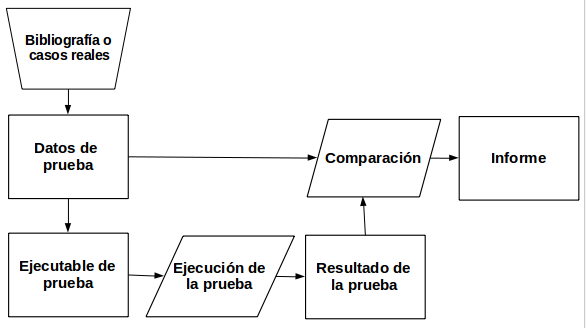
\includegraphics[width=0.9\textwidth]{imagenes/metodoprueba}}
  \caption{Esquema de la metodología para realizar las pruebas de unidad sobre los módulos.}
  \label{fig:metodoprueba}
\end{figure}

A medida que se desarrollaba un nuevo m\'odulo, se realizaban los casos de prueba para ese m\'odulo y una prueba de integraci\'on, que incorporaba todos los m\'odulos hasta el momento verificados.

\paragraph*{TleAdmin y CDM}
Dado que tanto los TLE como los CDM son los elementos fundamentales que dan inicio al an\'alisis de la probabilidad de colisi\'on, es fundamental tener un control sobre la correcta adquisici\'on de estos inputs. Sobre ellos se diseñaron pruebas funcionales. Se prueba siempre que los TLE de ambos objetos hayan sido adquiridos; si esto no fuera as\'i ya sea por complicaciones en la conexi\'on a internet, o porque los TLE para las fechas solicitadas no est\'an disponibles, el software interrumpe el proceso e indica a cu\'al de las situaciones se debe el problema. Mientras que para el caso de los CDM, el programa se interrumpe si el archivo ingresado no respeta el formato .xml capaz de procesar y anuncia un mensaje de alerta cuando el CDM a sido procesado pero no todos los campos de inter\'es se encuentran en \'el. 

\paragraph*{Comparar y SistReferencia}
Las pruebas realizadas para garantizar los correctos procedimientos respecto de la propagaci\'on y las transformaciones de los sistemas de referencia fueron fundamentales, pero s\'olo se realizaron en las primeras etapas del desarrollo, ya que no dependen de cada ejecuci\'on en particular, sino de la correcta implementaci\'on de los algoritmos.  

\paragraph*{Estad\'istica}
Para verificar la correcta implementaci\'on del m\'etodo de Osweiler para la generaci\'on de las matrices de covarianza, se gener\'o un caso de prueba que permite comparar los resultados con los que se publican en el trabajo del autor. Dada la dependencia de este m\'odulo con el m\'odulo de administraci\'on de los TLE, es importante que esta prueba es naturalmente de integraci\'on y es muy importante que se realice frecuentemente.

\paragraph*{Comparar y CodsAdmin}
El procedimiento que se realiza para la generaci\'on de la matriz de propagaci\'on de errores involucra la utilizaci\'on de los datos de misi\'on (o Datos de CODS). Esta tarea fue realmente compleja y se realizaron varias ejecuciones de la prueba sobre la manipulaci\'on de estos datos, ya que los mismos muchas veces no respetaban un formato estandarizado por ejemplo sobre las fechas o conten\'ian intervalos sin datos significativos, etc. Estas verificaciones se realizaron una sola vez hasta lograr que los datos resultaran ordenados dentro del per\'iodo de an\'alisis que se utiliz\'o para generar la matriz de propagaci\'on de errores. Por cuestiones de tiempo no se implement\'o una verificaci\'on automatizada sobre estos inputs, lo que debe ser tenido en cuenta si se desean generar matrices de propagaci\'on de errores actualizadas o en forma din\'amica (Fig. \ref{fig:pruebaCods} ).

\begin{figure}[!h]
 \centering
 \fbox{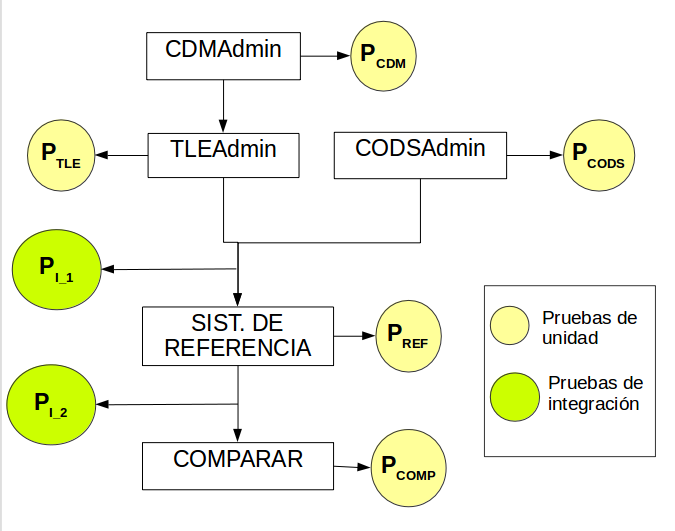
\includegraphics[width=0.6\textwidth]{imagenes/pruebasCods}}
 \caption[Casos de Prueba I]{Casos de prueba para los módulos que interactúan con los datos de Misión.}
 \label{fig:pruebaCods}
\end{figure}

\paragraph*{Encuentro}
Las pruebas realizada en el m\'odulo para la estimaci\'on de las probabilidades de colisi\'on tienen tambi\'en una fuerte dependencia del m\'odulo que gestiona los TLE, mientras que pueden configurarse o no para que la matriz de covarianza que utilizan sea generada por el m\'odulo de Osweiler o no. Salvo para el caso del m\'etodo de Lei-Chen, ya que en su trabajo existe un ejemplo que indica todos los par\'ametros que se utilizan en la ecuaci\'on final, y entonces se puede hacer una prueba s\'olo para esa unidad (Fig. \ref{fig:pruebaEncuentro}).

\begin{figure}
 \centering
 \fbox{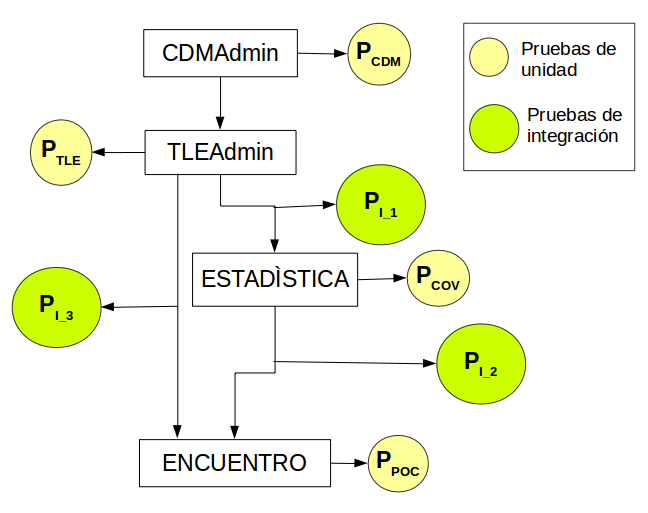
\includegraphics[width=0.6\textwidth]{imagenes/pruebasEncuentro}}
 \caption[Casos de Prueba II]{Casos de prueba del bloque completo, desde los inputs hasta el cálculo de la PoC.}
 \label{fig:pruebaEncuentro}
\end{figure}

\paragraph{Aplicaci\'on}
En lo que respecta a la aplicaci\'on que nuclea y despliega la interfaz gr\'afica, se realizaron inspecciones para depurar la correcta inicializaci\'on de variables y el flujo de las distintas vistas. 




\subsubsection*{Validaci\'on}

Al tratarse de un sistema que implementa distintas metodolog\'ias para el c\'alculo de par\'ametros, el control m\'as exhaustivo se bas\'o en analizar que los resultados de los algoritmos implementados fueran coherentes y coincidieran con los que exist\'ian en publicaciones bibliogr\'aficas o situaciones reales que se pod\'ian reproducir. \\

En conclusi\'on se han realizado distintas pruebas e inspecciones, pero no pruebas exhaustivas.
Un desarrollo detallado de los resultados de las pruebas y validaciones se describe en la Sec. \ref{chap:resultados}\\

\section{Gesti\'on de la Configuraci\'on}

Para la gesti\'on de la configuraci\'on se utiliz\'o el repositorio Git (Ver Sec. \ref{sec:entorno}) para el control de versiones, al que d\'ia a d\'ia se incorporaba el proyecto. El proyecto fue estructurado en distintos directorios que agrupan m\'odulos con los c\'odigos fuente y los inputs del sistema; y a su vez un directorio denominado TESIS, donde se almacena, fundamentalmente este escrito y otros documentos con las especificaciones del sistema, el dise\~no y la arquitectura.  

Se consideraron bajo control de configuraci\'on los siguientes elementos:

\begin{itemize}
 \item Especificaciones del Sistema.
 \item Inputs: TLE, CDM y archivos CODS.
 \item Dise\~no y arquitectura.
 \item C\'odigo fuente.
 \item Documento de TESIS.
\end{itemize}

\subsubsection*{Especificaciones del Sistema}
Si bien no se plasman en una documentaci\'on rigurosa, las especificaciones fueron revisadas en las distintas reuniones con el director y la codiretora del trabajo.

\subsubsection*{Inputs: TLE, CDM y archivos CODS}
Se crearon directorios espec\'ificos para cada uno de los archivos de entrada: TLE, CDM y archivos CODS, para garantizar que los inputs utilizados en los procesos de V\&V sean siempre los correctos y los mismos. 

\subsubsection*{Dise\~no y arquitectura}
Los distintos documentos de dise\~no y de arquitectura se almacenan en el directorio TESIS, y sus nomenclaturas hacen referencia a la fecha correspondiente al desarrollo. 

\subsubsection*{C\'odigo fuente}
En todas las actualizaciones diarias del proyecto, siempre que existieran cambios sobre los c\'odigos fuente, en las identificaciones de la actualizaci\'on se plasm\'o el c\'odigo fuente que se modific\'o y una referencia al tipo de modificaci\'on que se realiz\'o.\\


En general, se realizaron {\it{commits}} diarios. Mediante este proceso los cambios eran actualizados en el proyecto con un mensaje de identificaci\'on de la actualizaci\'on. Si bien no se sigui\'o una nomenclatura formal para estas actualizaciones, siempre se mencionaron los distintos archivos modificados con una muy breve nota sobre el cambio realizado.  

Se paut\'o realizar un release una vez por mes, ya que era la frecuencia con la que se planific\'o que existieran nuevos m\'odulos y pruebas de unidad y/o de integraci\'on. 

